\section{Aufgabe 7 - Datenübertragung mittels Infra-Rot (IR)}
\label{sec:aufgabe-7---datenuebertragung-mittels-infra-rot-ir}

In dieser Aufgabe soll eine Datenübertragung mittels Infrarotsignal implementiert werden.
Um ein solches Signal in der verwendeten Simulationssoftware zu simulieren, wurde die Schaltung aus Abbildung \ref{fig:a7-simulation-infrarot} verwendet.

\begin{figure}[h]
    \centering
    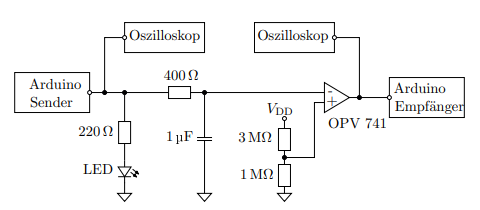
\includegraphics{pictures/a7-addon.png}
    \caption{Simulation eines Infrarotsignals}
    \label{fig:a7-simulation-infrarot}
\end{figure}

Für diese Aufgabe, soll ein 38kHz Signal von einem Sender-Mikrocontroller and einen Empfänger-Mikrocontroller gesendet werden.
Eine Übertragung von Text soll mithilfe des Sendens von Morsezeichen implementiert werden.
Es soll dem Benutzer dann ermöglicht werden, über die serielle Schnittstelle Zeichen an den Sender zu übergeben.
Dieser sendet die Zeichen dann an den Empfänger, welche sie wieder ausgibt.

\newpage

\subsection{Materialien}
\label{subsec:a7-materialien}

\begin{table}[ht]
    \centering
    \caption{Aufgabe 7 - Verwendete Materialien}
    \label{tab:a7-materialien}
    \begin{tabular}{| l | l | l |}
        \hline
        Bezeichnung & Eigenschaften & Menge \\
        \hline
        LED & Rot & 1 \\
        Widerstand & $220\Omega$ & 1 \\
        & Rot - Rot - Braun - Gold & \\
        Widerstand & $400\Omega$ & 1 \\
        & Gelb - Schwarz - Braun - Gold & \\
        Widerstand & $1M\Omega$ & 1 \\
        & Braun - Schwarz - Grün - Gold & \\
        Widerstand & $3M\Omega$ & 1 \\
        & Orange - Schwarz - Grün - Gold & \\
        Kondensator & $10 \mu F$ - 1 \\
        Operationsverstärker & & 1 \\
        (optional) Oszilloskop & & 2\\
        Mikrocontroller & Arduino Uno R3 & 2 \\
        \hline
    \end{tabular}
\end{table}

\subsection{Vorbereitung}
\label{subsec:a7-vorbereitung}

\subsubsection{Aufgabe 1}

Zur Codierung von Buchstaben in Morsecode soll recherchiert werden, wie diese Codierung erfolgt.
Es werden sogenannte \textit{dit}s und \textit{dah}s verwendet \cite{morsecode}.
Ein \textit{dit} wird als Punkt und ein \textit{dah} als Strich symbolisiert.
Des weiteren wird nicht zwischen Groß- und Kleinbuchstaben unterschieden.
In Tabelle \ref{tab:a7-morsecode} werden die Zuordnung zwischen Buchstaben und Morsecode gezeigt.

\begin{table}[h]
    \centering
    \caption{Morsecode von Buchstaben}
    \label{tab:a7-morsecode}
    \begin{tabular}{| c | c | c | c | c | c |}
        \hline
        Buchstabe & Code & Buchstabe & Code & Buchstabe & Code \\
        A & * - & J & * - - - & S & * * * \\
        B & - * * * & K & - * - & T & - \\
        C & - * - * & L & * - * * & U & * * - \\
        D & - * * & M & - - & V & * * * - \\
        E & * & N & - * & W & * - - \\
        F & * * - * & O & - - - & X & - * * - \\
        G & - - * & P & * - - * & Y & - * - - \\
        H & * * * * & Q & - - * - & Z & - - * * \\
        I & * * & R & * - * & &  \\
        \hline
    \end{tabular}
\end{table}

\newpage

\subsubsection{Aufgabe 2}

Es soll überlegt werden, wie das Einlesen von Zeichen und die Codierung dieser mittels eines Mikrocontroller efolgen könnte.

Zuerst kann ein Buchstabe mittels $Serial.read()$ eingelesen werden.
Durch die Verwendung einer Matrix, welche die Kodierung abbildet, kann ein Buchstabe kodiert werden.
Man kann dann ein Signal für die Dauer $t$ an einen Ausgangspin anlegen um ein dit zu senden.
Um ein dah zu senden, kann das Signal für die Dauer $3t$ anliegen.

\subsubsection{Aufgabe 3}

Es soll der benötigte Vorwiderstand der Infrarot-LED berechnet werden.
Dazu sind folgende Werte gegeben:

\begin{align}
    U = 5V \\
    I_D = 130mA \\
    U_D = 1,6V \\
    R_{on} = 14\Omega
\end{align}

\begin{figure}[h]
    \centering
    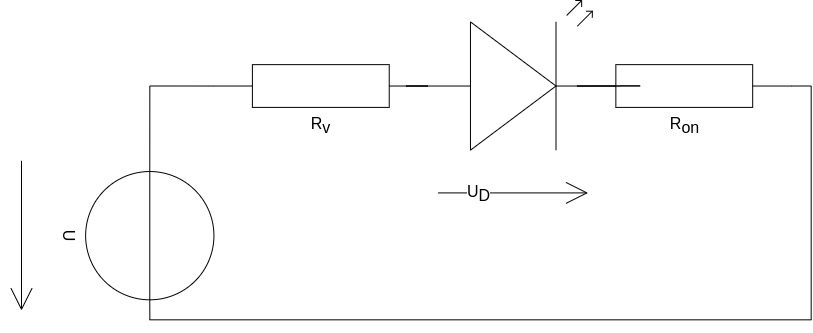
\includegraphics[height=0.3\textheight]{pictures/a7-rechnung-vorwiderstand.png}
    \caption{Angenommene Schaltung}
    \label{fig:a7-angenommene-schaltung}
\end{figure}

Gesucht ist der Widerstand $R_v$.
Zur Berechnung wurde die Schaltung aus Abbildung \ref{fig:a7-angenommene-schaltung} angenommen.

\begin{align}
    U_T = R_{on} * I_D \\
    = 14\Omega * 0,13A \\
    = 1,82V
\end{align}

\begin{align}
    U_{RV} = U - U_T - U_D \\
    = 5V - 1,82V - 1,6V \\
    = 1,58V
\end{align}

\begin{align}
    R_v = \frac{U_{RV}}{I_D} \\
    = \frac{1,58V}{0,13A} \\
    \underline{\underline{= 12,154\Omega}}
\end{align}

Der errechnete Vorwiderstand beträgt $12,154\Omega$, daher wird der $10\Omega$ Widerstand aus der E6-Reihe verwendet.

\subsection{Praktikumsaufgabe}
\label{subsec:a7-praktikumsaufgabe}

In Abbildung \ref{fig:a6-implementierung} ist die implementierte Schaltung abgebildet.
Links ist der sendende Mikrocontroller, rechts der Empfangende platziert.
Der Pin 11 wurde bei beidem als Aus- bzw.\ Eingang verwendet, da dieser PWM-Modulation unterstützt.
Die PWM-Unterstützung ist hier nicht notwendig, mehr dazu in der Fehlerdiskussion.

\begin{figure}[h]
    \centering
    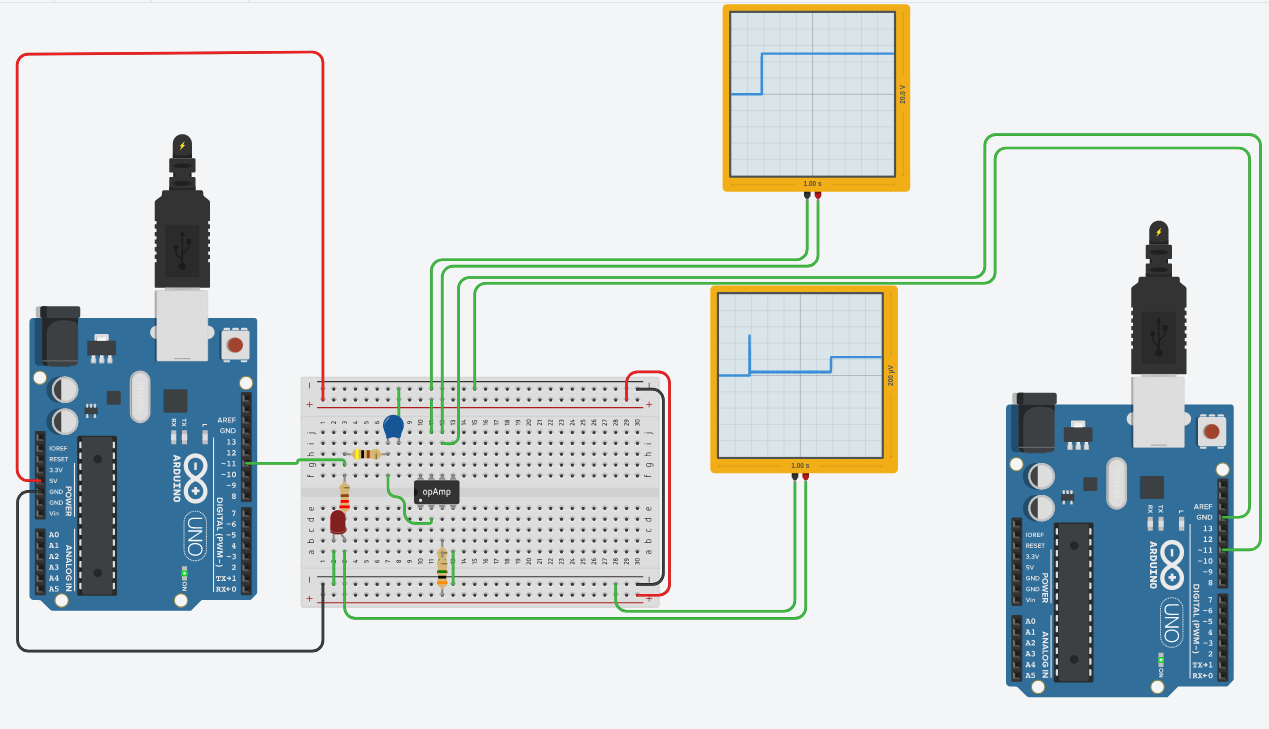
\includegraphics[width=\textwidth]{pictures/a7-praktik.png}
    \caption{Implementierte Schaltung für Aufgabe 7}
    \label{fig:a7-implementierung}
\end{figure}

Im nachfolgenden Text wird der Programmcode der Aufgabe erläutert.
Einzelne Teile des Codes werden ausgewählt und beschrieben.
Am Ende der jeweiligen Sektionen befinden sich die vollständigen Programmcodes des Senders und des Empfängers.

\newpage

\subsubsection{Sender}

\begin{lstlisting}[language=C,label={lst:a7-sender-wichtige-konstanten}, caption={Wichtige Konstanten des Senders}]
const unsigned long DURATION = 25;

const int PIN_SENDER = 11;

/*
1 - short
3 - long
-1 - NOP

NOP is needed since it's complex to work with jagged arrays in C
*/
const int CODE[26][4] = {
  {1, 3, -1, -1}, 	// A
  {3, 1, 1, 1}, 	// B
  {3, 1, 3, 1},		// C
  {3, 1, 1, -1},	// D
  {1, -1, -1, -1}, 	// E
  {1, 1, 3, 1}, 	// F
  {3, 3, 1, -1}, 	// G
  {1, 1, 1, 1}, 	// H
  {1, 1, -1, -1}, 	// I
  {1, 3, 3, 3}, 	// J
  {3, 1, 3, -1}, 	// K
  {1, 3, 1, 1}, 	// L
  {3, 3, -1, -1},	// M
  {3, 1, -1, -1}, 	// N
  {3, 3, 3, -1}, 	// O
  {1, 3, 3, 1}, 	// P
  {3, 3, 1, 3}, 	// Q
  {1, 3, 1, -1},	// R
  {1, 1, 1, -1}, 	// S
  {3, -1, -1, -1}, 	// T
  {1, 1, 3, -1}, 	// U
  {1, 1, 1, 3}, 	// V
  {1, 3, 3, -1}, 	// W
  {3, 1, 1, 3}, 	// X
  {3, 1, 3, 3}, 	// Y
  {3, 3, 1, 1}, 	// Z
};

const int OFFSET = 'A';
\end{lstlisting}

\newpage

In Listing \ref{lst:a7-sender-wichtige-konstanten} werden die verwendeten Konstanten gezeigt.
Die Konstante $DURATION$ wird verwendet, um die Zeit für dits und dahs zu berechnen.
In der $CODE$ Matrix ist die Kodierung von Buchstaben zu Morsecode abgebildet.
Dabei werden dits mit 1 und dahs mit 3 beschrieben.
In C ist ein jagged Array, d.h.\ ein Array, bei dem die Zeilen unterschiedliche Längen haben, nicht trivial zu erstellen.
Daher werden nicht verwendete Positionen mit -1 angegeben.
Die Konstante $OFFSET$ speichert den ASCII-Wert des Buchstaben 'A'.

\begin{lstlisting}[language=C,label={lst:a7-sender-schleife}, caption={Programmschleife des Senders}]
void loop() {
  if(Serial.available()) {
    send_letter(Serial.read());
  }
}

bool send_letter(char letter) {
  if (letter >= 'a' && letter <= 'z') {
    // If letter is lower case, set to uppercase
    letter -= 32;
  } else if (letter < 'A' || letter > 'Z') {
    return false;
  }

  Serial.println(letter);
  // Normalize to 0 - 25;
  int index = letter - 'A';
  for (int i = 0; i < 4; i++) {
    int multiplier = CODE[index][i];

    if (CODE[index][i] > -1) {
      digitalWrite(PIN_SENDER, HIGH);
      delay(DURATION * multiplier);
      digitalWrite(PIN_SENDER, LOW);
      delay(DURATION);
    } else {
      digitalWrite(PIN_SENDER, HIGH);
      delay(DURATION * 4);
      digitalWrite(PIN_SENDER, LOW);
      delay(DURATION);
      // Exit loop after end of code
      break;
    }
  }
  digitalWrite(PIN_SENDER, LOW);
  return true;
}
\end{lstlisting}

Die Programmschleife samt Hilfsmethode ist in Listing \ref{lst:a7-sender-schleife} dargestellt.
Die Schleife selbst liest nur einen Buchstaben vom seriellen Interface und übergibt diesen an die Funktion $send\_letter$.

Im ersten Teil der Hilfsmethode wird zuerst überprüft, ob der Buchstabe ein Kleinbuchstabe ist.
Ist dies der Fall, wird er zu einem Großbuchstaben umgewandelt.
Die Umwandlung wird durch Subtraktion des Unterschieds zwischen dem ASCII-Wert von 'a' und 'A' durchgeführt.
Sollte der Buchstabe weder ein Klein- noch ein Großbuchstabe sein, wird die Routine beendet.

Danach wird der benötigte Index der Kodierungsmatrix berechnet, indem vom ASCII-Wert des übergeben Buchstaben der Wert von 'A' abgezogen wird.
Dies normalisiert den Wert auf den Bereich $0 \leq index < 26$.
Die Zeile am entsprechenden Index wird sodann durchiteriert.
Ist der gespeicherte Wert an der Stelle $[index][i]$ größer als der definierte Platzhalter von -1, wird ein Morsecode gesendet.
Der Wert der Matrix dient dazu als Multiplikator der Zeitspanne, für die ein $HIGH$-Signal an Pin 11 angelegt wird.
Wird das Ende der Zeile, d.h.\ -1, erreicht, wird ein $HIGH$-Signal für die Zeit von $4*DURATIOn$ angegelegt, um das Ende des Signals zu markieren.
Abschließend wird die Schleife beendet und Pin 11 auf $LOW$ geschaltet.

\begin{lstlisting}[language=C,label={lst:a7-sender-programmcode}, caption={Vollständiger Programmcode des Senders der Aufgabe 7}]
const unsigned long DURATION = 25;

const int PIN_SENDER = 11;

/*
1 - short
3 - long
-1 - NOP

NOP is needed since it's complex to work with jagged arrays in C
*/
const int CODE[26][4] = {
  {1, 3, -1, -1}, 	// A
  {3, 1, 1, 1}, 	// B
  {3, 1, 3, 1},		// C
  {3, 1, 1, -1},	// D
  {1, -1, -1, -1}, 	// E
  {1, 1, 3, 1}, 	// F
  {3, 3, 1, -1}, 	// G
  {1, 1, 1, 1}, 	// H
  {1, 1, -1, -1}, 	// I
  {1, 3, 3, 3}, 	// J
  {3, 1, 3, -1}, 	// K
  {1, 3, 1, 1}, 	// L
  {3, 3, -1, -1},	// M
  {3, 1, -1, -1}, 	// N
  {3, 3, 3, -1}, 	// O
  {1, 3, 3, 1}, 	// P
  {3, 3, 1, 3}, 	// Q
  {1, 3, 1, -1},	// R
  {1, 1, 1, -1}, 	// S
  {3, -1, -1, -1}, 	// T
  {1, 1, 3, -1}, 	// U
  {1, 1, 1, 3}, 	// V
  {1, 3, 3, -1}, 	// W
  {3, 1, 1, 3}, 	// X
  {3, 1, 3, 3}, 	// Y
  {3, 3, 1, 1}, 	// Z
};

const int OFFSET = 'A';

void setup()
{
  Serial.begin(115000);
  pinMode(PIN_SENDER, OUTPUT);
}

void loop()
{
  if(Serial.available()) {
    send_letter(Serial.read());
  }
}

bool send_letter(char letter) {
  if (letter >= 'a' && letter <= 'z') {
    // If letter is lower case, set to uppercase
    letter -= 32;
  } else if (letter < 'A' || letter > 'Z') {
    return false;
  }

  Serial.println(letter);
  // Normalize to 0 - 25;
  int index = letter - 'A';
  for (int i = 0; i < 4; i++) {
    int multiplier = CODE[index][i];

    if (CODE[index][i] > -1) {
      digitalWrite(PIN_SENDER, HIGH);
      delay(DURATION * multiplier);
      digitalWrite(PIN_SENDER, LOW);
      delay(DURATION);
    } else {
      digitalWrite(PIN_SENDER, HIGH);
      delay(DURATION * 4);
      digitalWrite(PIN_SENDER, LOW);
      delay(DURATION);
      // Exit loop after end of code
      break;
    }
  }

  digitalWrite(PIN_SENDER, LOW);
  return true;
}
\end{lstlisting}

\subsubsection{Empfänger}

\begin{lstlisting}[language=C,label={lst:a7-receiver-loop}, caption={Programmschleife des Empfängers}]
void loop()
{
    int value = digitalRead(PIN_RECEIVER);
    if(value == LOW && start_time <= 0) {
        start_time = millis();
    } else if (value == HIGH && start_time > 0) {
        unsigned long duration = millis() - start_time;
        int decoded = decode(millis() - start_time);
        start_time = 0;
        if (decoded > -1) {
            Serial.println((char)(decoded + OFFSET));
        }
    }
}
\end{lstlisting}

In Listing \ref{lst:a7-receiver-loop} ist die Programmschleife des Empfängers abgebildet.
Zuerst wird der Zustand des Pin 11 gelesen.
Ist der Zustand $LOW$, wird ein Timer gestartet.
Ändert sich der Zustand, wird die vergangene Zeit gemessen und dekodiert.
Der Timer wird zurückgesetzt und, sollte das Dekodieren erfolgreich gewesen sein, wird der empfangenen Buchstabe auf der seriellen Schnittstelle ausgegeben.

\newpage

\begin{lstlisting}[language=C,label={lst:a7-receiver-decode}, caption={Dekodieren empfangenen Daten}]
int decode(unsigned long duration) {
  int result = -1;
  if (duration > DURATION*4 - DURATION_THRESHOLD &&
      duration < DURATION*4 + DURATION_THRESHOLD) {
    current_code[current_code_index] = -1;
    for(int i = 0; i < 26; i++) {
      for(int j = 0; j < 4; j++) {
        if(CODE[i][j] == current_code[j]) {
          if(CODE[i][j] == -1) {
            // Set result if codes match until end
            result = i;
          }
        } else {
          break;
        }
      }
    }

    // Reset code
    for(int i = 0; i < 4; i++) {
      current_code[i] = -1;
    }
    current_code_index = -1;
  } else if (duration > DURATION*3 - DURATION_THRESHOLD &&
      duration < DURATION*3 + DURATION_THRESHOLD) {
    current_code[current_code_index] = 3;
  } else if (duration > DURATION - DURATION_THRESHOLD &&
      duration < DURATION + DURATION_THRESHOLD) {
    current_code[current_code_index] = 1;
  }
  current_code_index++;

  // Return -1 if encoding not possible
  return result;
}
\end{lstlisting}

\newpage

Das eigentliche Dekdoieren wird in Listing \ref{lst:a7-receiver-decode} vorgenommen.
Ist die Zeit zwischen einen Zustandswechsel vier mal $DURATION$, d.h.\ 100ms, wird der Buchstabe als Empfangen angenommen.
Durch vergleichen der Empfangenen dits und dahs wird der Buchstabe aus der Kodierungsmatrix gesucht.
Sollte das Ergebnis dekodiert werden können, so wird dieser in der Variable $result$ gespeichert.
Danach wird die Variable, die die empfangene Dits und Dahs zwischenspeichert, zurückgesetzt.
Ist die Zeit zwischen den Zustandswechseln $3*DURATION$ oder $DURATION$, wird jeweils ein Dah oder Dit in die Variable $current_code$ zwischengespeichert.
Schlussendlich wird das Ergebnis zurückgegeben, oder -1 wenn das Dekodieren nocht nicht oder nicht möglich ist.

\begin{lstlisting}[language=C,label={lst:a7-receiver-programmcode}, caption={Vollständiger Programmcode des Empfängers der Aufgabe 7}]
const unsigned long DURATION = 25;
const unsigned long DURATION_THRESHOLD = 5;

const int PIN_RECEIVER = 11;

/*
1 - short
2 - long
-1 - NOP

NOP is needed since it's complex to work with jagged arrays in C
*/
const int CODE[26][4] = {
  {1, 3, -1, -1}, 	// A
  {3, 1, 1, 1}, 	// B
  {3, 1, 3, 1},		// C
  {3, 1, 1, -1},	// D
  {1, -1, -1, -1}, 	// E
  {1, 1, 3, 1}, 	// F
  {3, 3, 1, -1}, 	// G
  {1, 1, 1, 1}, 	// H
  {1, 1, -1, -1}, 	// I
  {1, 3, 3, 3}, 	// J
  {3, 1, 3, -1}, 	// K
  {1, 3, 1, 1}, 	// L
  {3, 3, -1, -1},	// M
  {3, 1, -1, -1}, 	// N
  {3, 3, 3, -1}, 	// O
  {1, 3, 3, 1}, 	// P
  {3, 3, 1, 3}, 	// Q
  {1, 3, 1, -1},	// R
  {1, 1, 1, -1}, 	// S
  {3, -1, -1, -1}, 	// T
  {1, 1, 3, -1}, 	// U
  {1, 1, 1, 3}, 	// V
  {1, 3, 3, -1}, 	// W
  {3, 1, 1, 3}, 	// X
  {3, 1, 3, 3}, 	// Y
  {3, 3, 1, 1}, 	// Z
};
int current_code[4] = {};
int current_code_index = 0;

const int OFFSET = 65;

int start_time = 0;

void setup()
{
  Serial.begin(115000);
  pinMode(PIN_RECEIVER, INPUT);
}

void loop()
{
  int value = digitalRead(PIN_RECEIVER);
  if(value == LOW && start_time <= 0) {
    start_time = millis();
  } else if (value == HIGH && start_time > 0) {
    unsigned long duration = millis() - start_time;
    int decoded = decode(millis() - start_time);
    start_time = 0;
    if (decoded > -1) {
      Serial.println((char)(decoded + OFFSET));
    }
  }
}

int decode(unsigned long duration) {
  int result = -1;
  if (duration > DURATION*4 - DURATION_THRESHOLD &&
      duration < DURATION*4 + DURATION_THRESHOLD) {
    current_code[current_code_index] = -1;
    for(int i = 0; i < 26; i++) {
      for(int j = 0; j < 4; j++) {
        if(CODE[i][j] == current_code[j]) {
          if(CODE[i][j] == -1) {
            // Set result if codes match until end
            result = i;
          }
        } else {
          break;
        }
      }
    }

    // Reset code
    for(int i = 0; i < 4; i++) {
      current_code[i] = -1;
    }
    current_code_index = -1;
  } else if (duration > DURATION*3 - DURATION_THRESHOLD &&
      duration < DURATION*3 + DURATION_THRESHOLD) {
    current_code[current_code_index] = 3;
  } else if (duration > DURATION - DURATION_THRESHOLD &&
      duration < DURATION + DURATION_THRESHOLD) {
    current_code[current_code_index] = 1;
  }
  current_code_index++;

  // Return -1 if encoding not possible
  return result;
}
\end{lstlisting}

\subsection{Fehlerdiskussion}
\label{subsec:a7-fehlerdiskussion}

Es hätte zur Übertragung von Daten ein analoger Pin verwendet werden sollen.
Die Verwendung eines PWM-Pins führt zu fehlerhaften Übertragungen und Implementationsfehlern.

Des weiteren konnte ein sinnvolles Debugging des Codes nicht durchgeführt werden.
Beim Simulieren von zwei Mikrocontrollern dauert das Simulieren von 100ms, in der verwendeten Software, mehrere Sekunden.
Eine manuelle bzw.\ visuelle Überprüfung der Funktionalität ist dabei praktisch nicht mehr durchführbar.

Schlussendlich wäre eine interessante Erweiterung oder Alternative dieser Aufgabe, die Verwendung einer Huffman Kodierung anstelle des Morsecodes.
Beim Morsecode wird ein Endzeichen benötigt, um Zeichen zu Unterscheiden.
Bei der Huffman-Kodierung ist kein Codewort der Prefix eines anderen.
Damit kann eine Dekodierung ohne Endwort durchgeführt werden, da es Eindeutig ist, wann ein Wort endet \cite{huffman}.
